% The parallelogram spanned by v and w, with signed area ad-bc.
% Source: book/tex/linalg/dets.tex (§ The determinant of a matrix).
\documentclass[border=2mm]{standalone}
\usepackage{tikz}
\usepackage{amsmath,amssymb}
\usetikzlibrary{arrows.meta}
\begin{document}
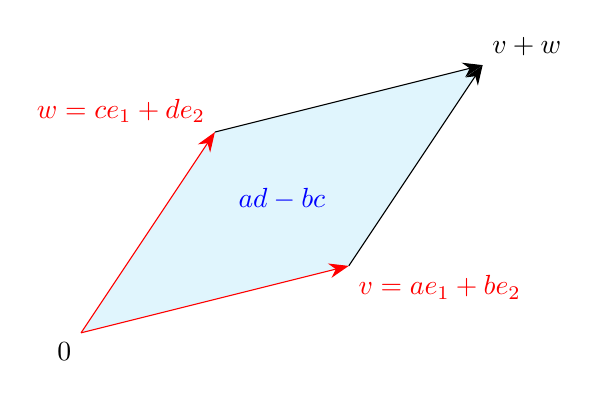
\begin{tikzpicture}[scale=0.85,>={Stealth[length=2.5mm]}]
  \coordinate (O) at (0,0);
  \coordinate (v) at (4,1);
  \coordinate (w) at (2,3);
  \coordinate (vw) at (6,4);
  \fill[cyan!12] (O)--(v)--(vw)--(w)--cycle;
  \draw[->,red] (O)--(v);
  \draw[->,red] (O)--(w);
  \draw[->] (v)--(vw);
  \draw[->] (w)--(vw);
  \node[below left] at (O) {$0$};
  \node[below right,red] at (v) {$v = ae_1 + be_2$};
  \node[above left,red] at (w) {$w = ce_1 + de_2$};
  \node[above right] at (vw) {$v+w$};
  \node[blue] at (3,2) {$ad-bc$};
\end{tikzpicture}
\end{document}
